\documentclass[11pt]{beamer}
\usepackage{listings} % Include the listings-package
\usepackage[T1]{fontenc}
\usepackage[utf8]{inputenc}
\usepackage[english]{babel}
\usepackage{amsmath}
\usepackage{amssymb, amsfonts, latexsym, cancel}
\usepackage{float}
\usepackage{graphicx} 
\usepackage{epstopdf}
\usepackage{subfigure}
\usepackage{hyperref}
%\usepackage{authblk}
\usepackage{blindtext}
\usepackage{booktabs} % Allows the use of \toprule, 
\usepackage{filecontents}
\usepackage{courier} %% Sets font for listing as Courier.
\usepackage{listings}
%\Plantilla del profesor 
\lstset{
tabsize = 2, %% set tab space width
showstringspaces = false, %% prevent space marking in strings, string is defined as the text that is generally printed directly to the console
numbers = left, %% display line numbers on the left
commentstyle = \color{green}, %% set comment color
keywordstyle = \color{blue}, %% set keyword color
stringstyle = \color{red}, %% set string color
rulecolor = \color{black}, %% set frame color to avoid being affected by text color
basicstyle = \small \ttfamily , %% set listing font and size
breaklines = true, %% enable line breaking
numberstyle = \tiny,
}
\usepackage{caption}
\DeclareCaptionFont{white}{\color{white}}
\DeclareCaptionFormat{listing}{\colorbox{gray}{\parbox{\textwidth}{#1#2#3}}}
\captionsetup[lstlisting]{format=listing,labelfont=white,textfont=white}
\definecolor{urlColor}{rgb}{0.06, 0.3, 0.57}
\definecolor{linkColor}{rgb}{0.57, 0.0, 0.04}
\definecolor{fileColor}{rgb}{0.0, 0.26, 0.26}
\hypersetup{
    colorlinks=true,
    linkcolor=linkColor,
    filecolor=fileColor,      
    urlcolor=urlColor,
}
\urlstyle{same}
\setbeamercovered{transparent}

\usetheme{CambridgeUS}
%\usetheme{Berkeley}
%\usetheme{Warsaw}
%\usetheme{Madrid}

\title[Arrays]{\bf\Huge 
-Arrays-}
%\Sorting algorithms and Search algorithms
\subtitle{Fundamentals to programming I}

\author[System Engineering School]
{
	Yeimy Estephany Huanca Sancho \inst{1}
	Omid Ernesto Chahuaris Choque \inst{2}
}
\institute[UNSA]
{
\inst{1}% 
System Engineering School\\
System Engineering and Informatic Department\\
Production and Services Faculty\\
San Agustin National University of Arequipa
}

\date[2020-04-08]{\scriptsize{2020-04-08}}
%\{
\includegraphics[width=3.0cm]{img/logo_unsa.jpg}}
\titlegraphic{
\includegraphics[width=6.0cm]{img/logo_unsa.jpg}}

\begin{document}

\begin{frame}
\titlepage
\end{frame}

\begin{frame}
\frametitle{Content}
\tableofcontents
\end{frame}

\section{Arrays}
\begin{frame}
\frametitle{Arrays-Definition}
\begin{itemize}
\item Also called arrangements.
\item Data structure containing a collection of data of the same type.
\end{itemize}
\end{frame}

\begin{frame}
\frametitle{Arrays-Properties}
\begin{itemize}
\item They are used as containers to store related data.
\item All the data included in the array is of the same type.
\item The size of the Array is established when it is created.
\item To access the Array data, the position it occupies within the set must be used.
\end{itemize}
\end{frame}

\begin{frame}
\frametitle{Arrays-Declaration}
\begin{itemize}
\item Square brackets are used to indicate that it is an Array and not a simple variable.
\

{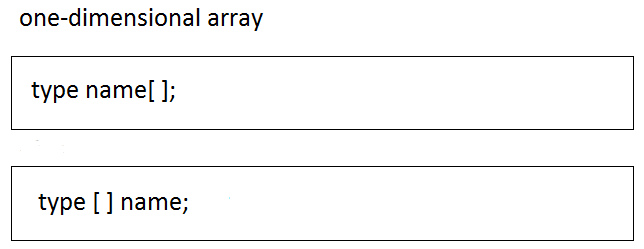
\includegraphics[width=7.0cm]{img/DeclarationA.png}}
{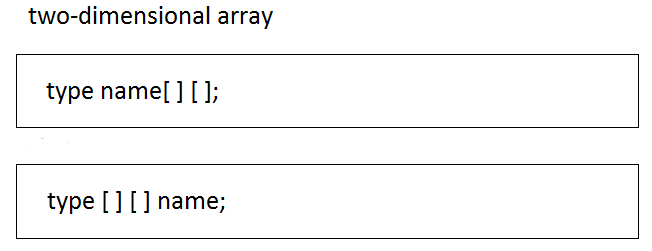
\includegraphics[width=7.0cm]{img/DeclarationB.png}}
\end{itemize}
\end{frame}

\begin{frame}
\frametitle{Arrays-Creation}
\begin{itemize}
\item They are created with the "new" operator.
\
{\includegraphics[width=7.0cm]{img/creation.png}}
\end{itemize}
\end{frame}

\begin{frame}
\frametitle{Arrays-Use}
\begin{itemize}
\item Indexes are used to access the elements of an array.
\
{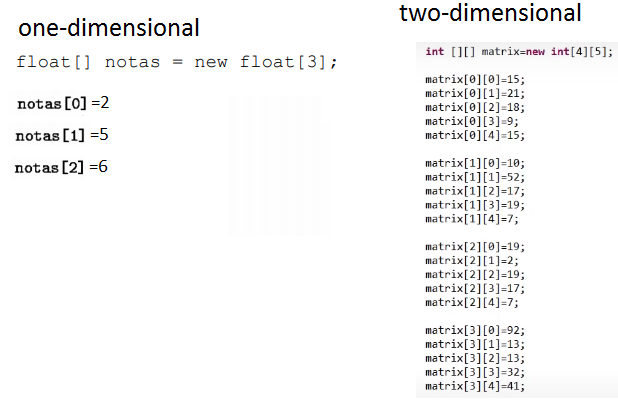
\includegraphics[width=7.0cm]{img/Arrays.png}}
\end{itemize}
\end{frame}

\begin{frame}
\frametitle{Arrays-Initialization in the declaration}
\begin{itemize}
\item You can assign an initial value to the elements of an Array in the declaration itself.

\centering
{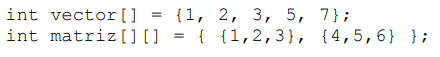
\includegraphics[width=8.0cm]{img/Inice.png}}
\end{itemize}
\end{frame}

\begin{frame}
\frametitle{Arrays-Manipulation Examples}
\begin{itemize}
\item Operations are done component by component.
{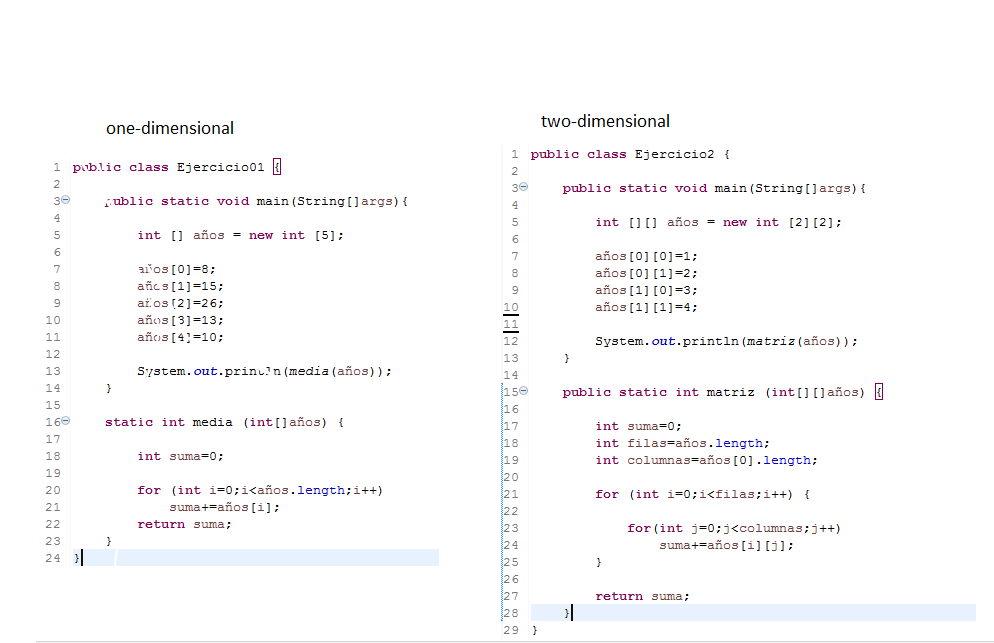
\includegraphics[width=10.0cm]{img/Examples.png}}
\end{itemize}
\end{frame}

\section{Character string}

\begin{frame}
\frametitle{Character string}
\begin{itemize}
\item The java.lang.String class is used to represent character strings in Java. It includes different methods that help us with character string operations.

\end{itemize}
\end{frame}

\begin{frame}
\frametitle{Character string-substring}
\begin{itemize}
\item The "substring" method allows us to get a substring.
\
{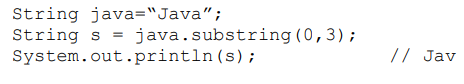
\includegraphics[width=10.0cm]{img/a1.png}}
\end{itemize}
\end{frame}

\begin{frame}
\frametitle{Character string-charAt}
\begin{itemize}
\item The "charAt (n)" method returns the character that is in position n of the string.
\
{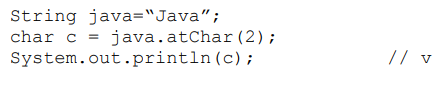
\includegraphics[width=10.0cm]{img/a2.png}}
\end{itemize}
\end{frame}

\begin{frame}
\frametitle{Character string-indexOf}
\begin{itemize}
\item The "indexOf (s)" method returns the position of a substring within a string.
\
{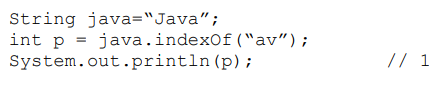
\includegraphics[width=10.0cm]{img/a3.png}}
\end{itemize}
\end{frame}

\begin{frame}
\frametitle{Character string-replace}
\begin{itemize}
\item The "replace (old, new)" method replaces substrings.
\
{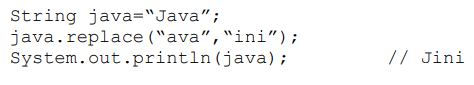
\includegraphics[width=10.0cm]{img/a4.png}}
\end{itemize}
\end{frame}

\begin{frame}
\frametitle{Character string-equals}
\begin{itemize}
\item The "equals (s)" method is used to  whether two strings are equals.
\
{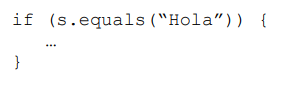
\includegraphics[width=8.0cm]{img/a5.png}}
\end{itemize}
\end{frame}

\begin{frame}
\frametitle{Character string-startsWith}
\begin{itemize}
\item The method "starts with (s)" tells us if a string starts with a certain prefix.
\

{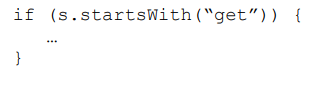
\includegraphics[width=8.0cm]{img/a6.png}}
\end{itemize}
\end{frame}

\begin{frame}
\frametitle{Character string-endsWith}
\begin{itemize}
\item The "endsWith (s)" method tells us if a string ends with a certain suffix.
\

{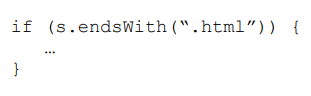
\includegraphics[width=8.0cm]{img/a7.png}}
\end{itemize}
\end{frame}

\begin{frame}
\frametitle{Character string-length}
\begin{itemize}
\item The "length" method tells us the length of the string
\
{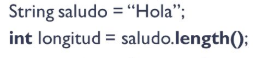
\includegraphics[width=8.0cm]{img/a8.png}}
\end{itemize}
\end{frame}


\section{Sorting algorithms}
\begin{frame}
\frametitle{Sorting algorithms}
\begin{itemize}
\item sort by selection.
\item insertion sort.
\item Direct exchange ordering (Bubblesort).
\item QuickSort
\end{itemize}
\end{frame}

\begin{frame}
\frametitle{Sorting algorithms }
\begin{itemize}
\item Selection sort
\begin{itemize}
\item Procedure: In each iteration, the smallest element of the unordered subset or subvector is selected and exchanged with the first element of this.
\item Greater efficiency
\item Complexity: n squared
\item Method: selection
\end{itemize}
\end{itemize}
\begin{center}
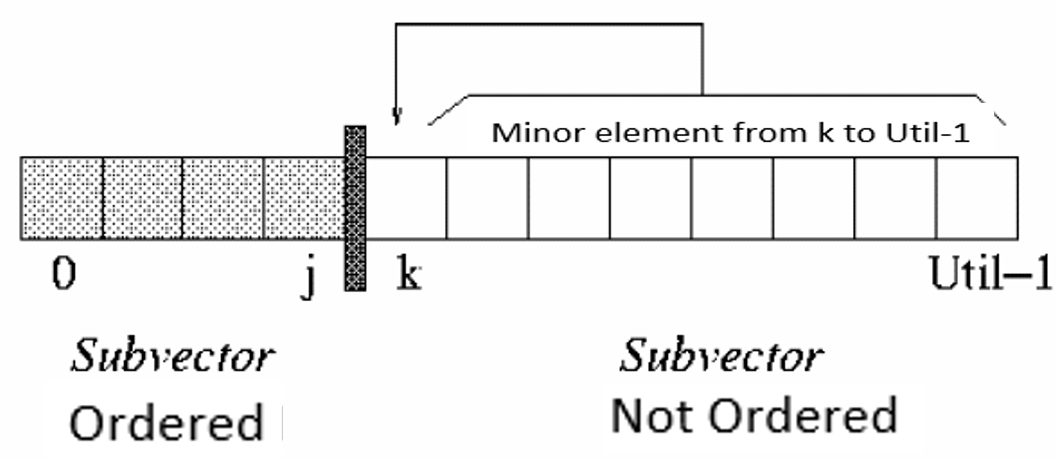
\includegraphics[width=7.0cm]{img/selec.png}
\end{center}
\end{frame}


\begin{frame}
\frametitle{Sorting algorithms}
\begin{itemize}
\item Insertion sort
\begin{itemize}
\item Procedure: In each iteration, an element from the unordered subvector is inserted at the correct position within the ordered subvector.
\item Greater efficiency
\item Complexity: n squared/2
\item Method: insert
\item Example: a deck of cards
\end{itemize}
\end{itemize}
\begin{center}
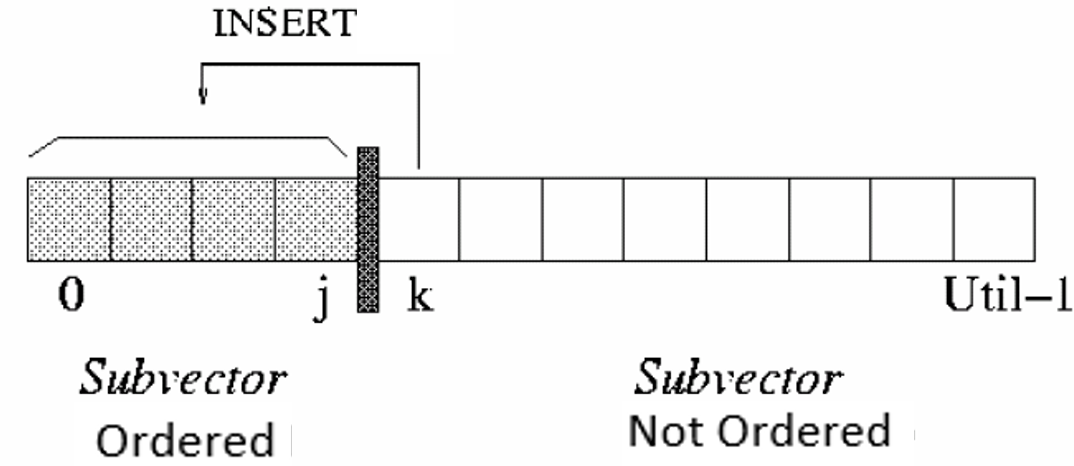
\includegraphics[width=7.0cm]{img/inser.png}
\end{center}
\end{frame}

\begin{frame}
\frametitle{Sorting algorithms}
\begin{itemize}
\item Direct exchange ordering (Bubblesort)
\begin{itemize}
\item Lower efficiency
\item Complexity: n squared
\item Method: exchange
\item Is more simple
\end{itemize}
\end{itemize}
\begin{center}
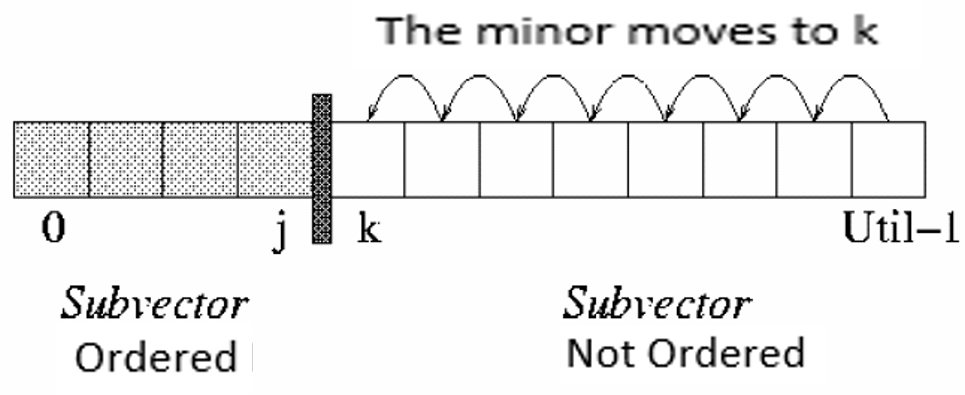
\includegraphics[width=7.0cm]{img/burbu.png}
\end{center}
\end{frame}

\begin{frame}
\frametitle{Sorting algorithms}
\begin{itemize}
\item QuickSort
\begin{itemize}
\item Procedure: Reposition the other elements of the list on each side of the pivot, so that on one side are all the lesser than him, and on the other the greater
\item Greater efficiency
\item Complexity: n log n or n squared in the worst case
\item Method: partition
\end{itemize}
\end{itemize}
\end{frame}

\section{Search algorithms}
\begin{frame}
\frametitle{Sorting algorithms}
\begin{itemize}
\item Linear search or Sequential search
\begin{itemize}
\item Process :It is compared sequentially, one by one.
\end{itemize}
\end{itemize}
\begin{center}
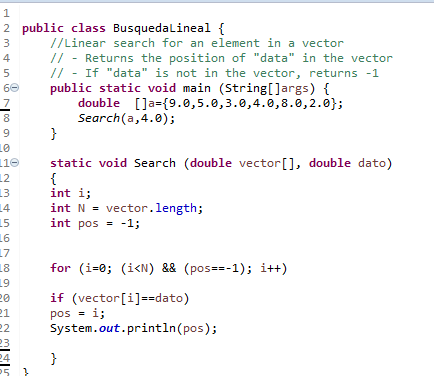
\includegraphics[width=7.0cm]{img/lineal (2).png}
\end{center}
\end{frame}

\begin{frame}
\frametitle{Sorting algorithms}
\begin{itemize}
\item Binary search
\begin{itemize}
\item Pre-condition: Must be ordered
\item Process :
\begin{itemize}
\item The searched data is compared with the element in the center of the vector
\item If they match, we have found the desired data.
\item If the data is greater than the central element of the vector, we have to find the data in the second half of the vector.
\item If the data is less than the central element of the vector, we have to find the data in the first half of the vector.
\end{itemize}
\end{itemize}
\end{itemize}
\end{frame}

\begin{frame}
\frametitle{Sorting algorithms}
\begin{itemize}
\item Binary search
\end{itemize}
\begin{center}
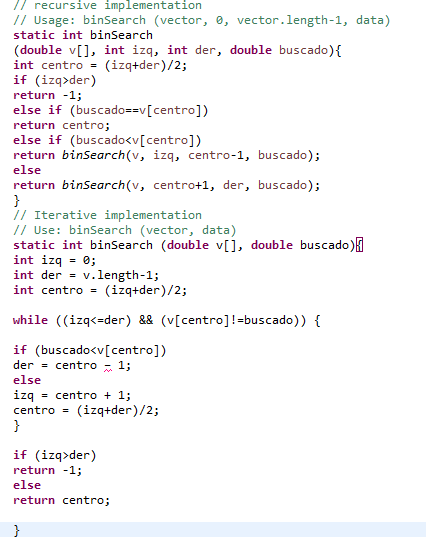
\includegraphics[width=7.0cm]{img/binaria (2).png}
\end{center}
\end{frame}

\section{Requirements}
\begin{frame}
\frametitle{Requirements}
\begin{itemize}
\item JDK >=1.8
\item MS Windows, MacOS, GNU/Linux: Oracle
\begin{itemize}
\item jdk-8u261-windows-i586.exe
\item jdk-8u261-windows-x64.exe
\item jdk-8u261-macosx-x64.dmg
\item jdk-8u261-linux-x64.tar.gz (Optional)
\end{itemize}
\item GNU/Linux: Ubuntu 
\end{itemize}
\end{frame}

\section{Code }
\begin{frame}
\frametitle{Code}
\begin{itemize}
\item Selection sort
\end{itemize}
\begin{center}
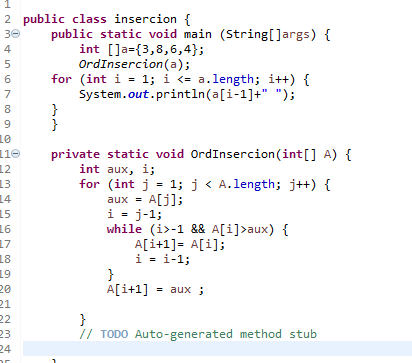
\includegraphics[width=8.0cm]{img/insercion (2).png}
\end{center}
\end{frame}

\begin{frame}
\frametitle{Code}
\begin{itemize}
\item Selection sort
\end{itemize}
\begin{center}
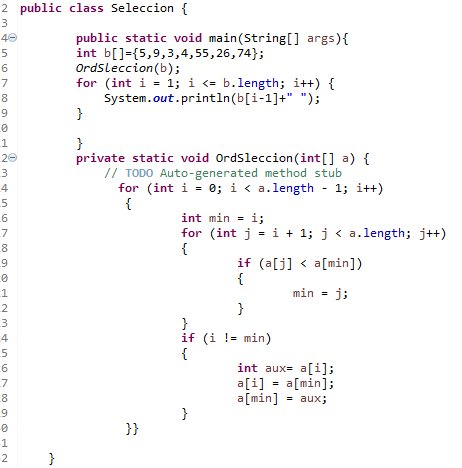
\includegraphics[width=8.0cm]{img/seleccion (2).png}
\end{center}
\end{frame}

\begin{frame}
\frametitle{Code}
\begin{itemize}
\item Insertion sort
\end{itemize}
\begin{center}
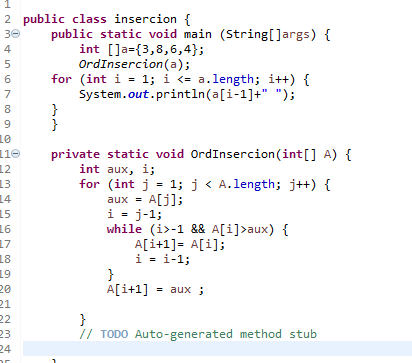
\includegraphics[width=8.0cm]{img/insercion (2).png}
\end{center}
\end{frame}

\begin{frame}
\frametitle{Code}
\begin{itemize}
\item Direct exchange ordering (Bubblesort)
\end{itemize}
\begin{center}
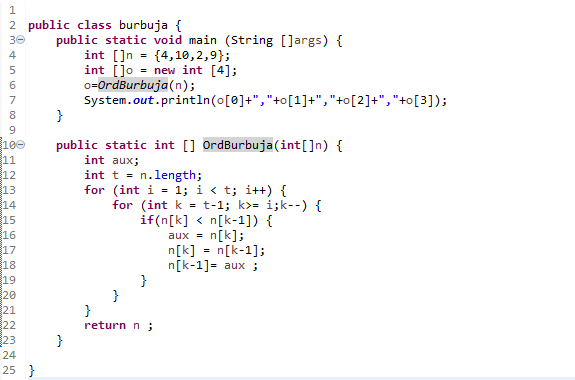
\includegraphics[width=10.0cm]{img/Met burbuja (2).png}
\end{center}
\end{frame}

\begin{frame}
\frametitle{Code}
\begin{itemize}
\item QuickSort
\end{itemize}
\begin{center}
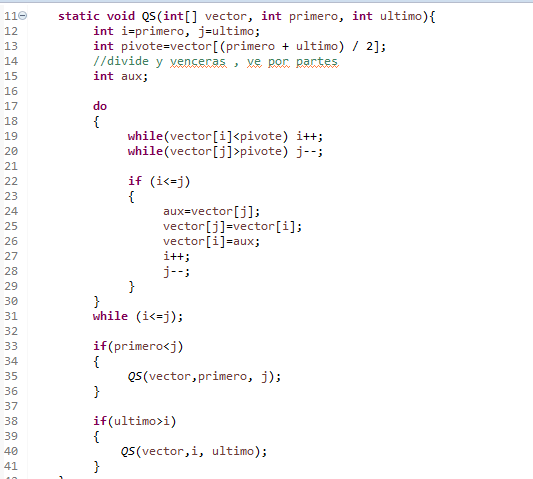
\includegraphics[width=8.0cm]{img/QS (2).png}
\end{center}
\end{frame}



\section{References}
\begin{frame}
\frametitle{References - Web pages}
\begin{itemize}
\item \url{https://elvex.ugr.es/decsai/java/}
\item \url{https://es.wikipedia.org/wiki/Algoritmo_de_ordenamiento}
\item \url{https://es.wikipedia.org/wiki/Quicksort}
\item \url{https://gl-epn-programacion-ii.blogspot.com/2010/06/metodos-de-ordenamiento.html}
\item \url{https://sites.google.com/a/espe.edu.ec/programacion-ii/home/a1-arreglos/algoritmos-de-ordenacion-y-busqueda}
\item \url{https://slideplayer.es/slide/1383043/}
\item \url{https://www.youtube.com/watch?v=_tUncS0AsNE}
\end{itemize}
\end{frame}

\begin{frame}
\frametitle{References - Books}
\begin{itemize}
\item { Java programming basics of Marco Aedo}
\end{itemize}
\end{frame}

\begin{frame}
\begin{center}
Thanks for your attention!...


\end{center}
\end{frame}

\end{document}
